\documentclass[10pt]{article}
\setlength{\topmargin}{-0.5in}
\setlength{\textwidth}{6.5in}
\setlength{\oddsidemargin}{0in}
\setlength{\textheight}{9in}

\newcommand{\wlin}{\mathbf{w}_{\text{lin}}}
\newcommand{\out}{\text{out}}
\newcommand{\val}{\text{val}}

%\usepackage{multirow}
%\usepackage{rotating}
\usepackage[fleqn]{amsmath}
\usepackage{natbib}
\usepackage{palatino}
\usepackage{url}
\usepackage{graphicx}

\usepackage[fleqn]{amsmath}
\usepackage{amsfonts}
\usepackage{mathtools}
\usepackage{natbib}
\usepackage{palatino}
\usepackage{url}
\usepackage{graphicx}

\DeclarePairedDelimiter\floor{\lfloor}{\rfloor}

\newcommand{\vecw}{{\mathbf{w}}}
\newcommand{\vecxn}{{\mathbf{x}_n}}

\begin{document}

\title{CSE 417T: Homework 3 Solution Sketches}



\maketitle

\noindent \textbf{Note:} These are not intended to be comprehensive,
just to help you see what the answers should be.

\begin{enumerate}

\item[Regularizations]

For part (a) First note that
  \[\nabla E_{\text{aug}} (\vec{w}) = \nabla (E_{\text{in}}
  (\vec{w} +\lambda \vec{w}^T \vec{w}) = \nabla E_{\text{in}}
  (\vec{w}) + 2 \lambda \vec{w} \]
  Thus, the weight update for gradient descent ($-\eta \nabla
  E_{\text{aug}} (\vec{w})$) becomes:
  \[ \vec{w} - \eta \nabla E_{\text{in}} (\vec{w}) + 2 \eta \lambda \vec{w} =
  \vec{w} (1 - 2\eta\lambda) - \eta \nabla E_{\text{in}} (\vec{w}) \]

Similarly for part (b), let $sign(\vec{w})$ be a vector denoting the sign of each element (let the sign of 0 be 0). 
We get that
\[
    \vec{w}(t+1) \leftarrow \vec{w}(t) - \eta\lambda sign(\vec{w}(t)) - \eta\nabla E_{\text{in}}(\vec{w}(t))
\]

For part (c), below are the reference results.
%[CJ: I have changed the descriptions slightly after the assignment is posted. So please give full points as long as the answers are close.]

\begin{center}
\begin{tabular}{l|c|c|c|c}
& \multicolumn{2}{c|}{$L_1$ Regularizer} & \multicolumn{2}{c}{$L_2$ Regularizer} \\
& Binary Error on Test Set & \# 0 in weights & Binary Error on Test Set & \# 0 in weights \\ \hline
$\lambda=0$ & - & - & 0.1028 & 8\\
$\lambda=0.0001$ & 0.0981 & 8 & 0.1028 & 8\\
$\lambda=0.001$ & 0.0935 & 15 & 0.0935 & 8\\
$\lambda=0.005$ & 0.0888 & 26 & 0.0981 & 8\\
$\lambda=0.01$ & 0.0794 & 36 & 0.0981  & 8\\
$\lambda=0.05$ & 0.1028 & 52 & 0.1168 & 8\\
$\lambda=0.1$ & 0.1355 & 57 & 0.1215 & 8\\
\end{tabular}
\end{center}


  There might be differences on the number of 0s depending whether students give some tolerance range to define 0. Please focus on the trend during grading.
  $L_1$ regularizer with truncated gradient tends to generate weights vectors with 0s. 
  This is helpful in reducing dimensions in high-dimensional learning.

\item[Exercise 4.5] 
(a) $\Gamma$ is the identify matrix.\\
(b) $\Gamma$ is a row vector with every element to be $1$.


\item[Problem 4.25 (a)-(c)]

For part (a), not necessarily. For example, a learner with low
validation error on a small validation set may just have gotten lucky
compared with a learner with a larger validation error on a larger
validation set.

For part (b), yes, because all the validation sets are the same. 

For part (c), let's index the error terms by the number of the
learning model. Then the event that $E_{\out}(m^*) > E_{\val}(m^*) +
\epsilon$ implies that either $E_{\out}(1) > E_{\val}(1) + \epsilon$
or $E_{\out}(2) > E_{\val}(2) + \epsilon$, $\ldots$, or $E_{\out}(M) >
E_{\val}(M) + \epsilon$. Applying the union bound, similarly to what
we did for the multiple hypotheses version of the Hoeffding
inequality, we get:
\[ \Pr [E_{\out}(m^*) > E_{\val}(m^*) + \epsilon] \leq \sum_{m=1}^{M}
\Pr [E_{\out}(m) > E_{\val}(m) + \epsilon] \leq \sum_{m=1}^{M} e^{-2
  \epsilon^2 K_m} \]
(where the second inequality comes from the one-sided version of
Hoeffding's inequality). From the definition of $\kappa (\epsilon)$,
$e^{-2 \epsilon^2 \kappa(\epsilon)} = \frac{1}{M} \sum_{m=1}^{M} e^{-2
  \epsilon^2 K_m}$. Therefore:
\[ \Pr [E_{\out}(m^*) > E_{\val}(m^*) + \epsilon] \leq M e^{-2
  \epsilon^2 \kappa(\epsilon)} \]

     
\item[5.4]
For (a), note that you didn't pick the best out of 500, you
effectively picked the best out of 50,000 because the S\&P first picked
the 500 for you. Therefore, you should use $M=50,000$ in the bound,
which would make the bound basically useless.

For (b), again we are getting sample selection bias (in this case by
snooping). We can't use the set of stocks currently in the S\&P 500,
we have to use those that were in there when the buy and hold strategy
would have started, 50 years ago. There is really nothing we can say
about buy and hold for general stock trading based on the current S\&P
500, we'd have to be sampling from the right set to start with.


%
%\item[ID3]
% 
%(a) The root node of the decision tree after running ID3 is ``Stripe''. 
%%Let $H(p)= p\log(1/p) + (1-p)\log(1/(1-p))$ be the entropy of binary signals in which one of the signals has probability $p$ in the distribution. 
%We can calculate the information gain for choosing each attribute. 
%
%The entropy of the data before splitting is
%$\frac{2}{5}\log\left(\frac{5}{2}\right)+\frac{3}{5}\log\left(\frac{5}{3}\right) \approx 0.971$.
%
%The average entropy after splitting using ``Color'' is
%$\frac{1}{5} \times 0 + \frac{4}{5} \left[ \frac{2}{4}\log\left(\frac{4}{2}\right) + \frac{2}{4}\log\left(\frac{4}{2}\right)\right] = 0.8$.
%
%The average entropy after splitting using ``Stripes'' is
%$\frac{2}{5} \times 0 + \frac{3}{5} \left[ \frac{1}{3}\log\left(\frac{3}{1}\right) + \frac{2}{3}\log\left(\frac{3}{2}\right)\right] \approx 0.551$.
%
%The average entropy after splitting using ``Texture'' is
%$\frac{2}{5} \left[\frac{1}{2}\log\left(\frac{2}{1}\right) + \frac{1}{2}\log\left(\frac{2}{1}\right)\right] + \frac{3}{5} \left[ \frac{1}{3}\log\left(\frac{3}{1}\right) + \frac{2}{3}\log\left(\frac{3}{2}\right)\right] \approx 0.951$.
%
%Given the above values, we have
%\begin{align*}
%Gain(D,\mbox{Color}) &\approx 0.971 - 0.8 = 0.171 \\
%Gain(D,\mbox{Stripes}) &\approx 0.971 - 0.551 = 0.420 \\ 
%Gain(D,\mbox{Texture}) &\approx 0.971 - 0.951 = 0.020 
%\end{align*}
%Therefore, splitting using ``Stripes'' leads to the maximum information gain.
%
%(b) The final decision tree looks like the following:
%\begin{figure}[h!]
%  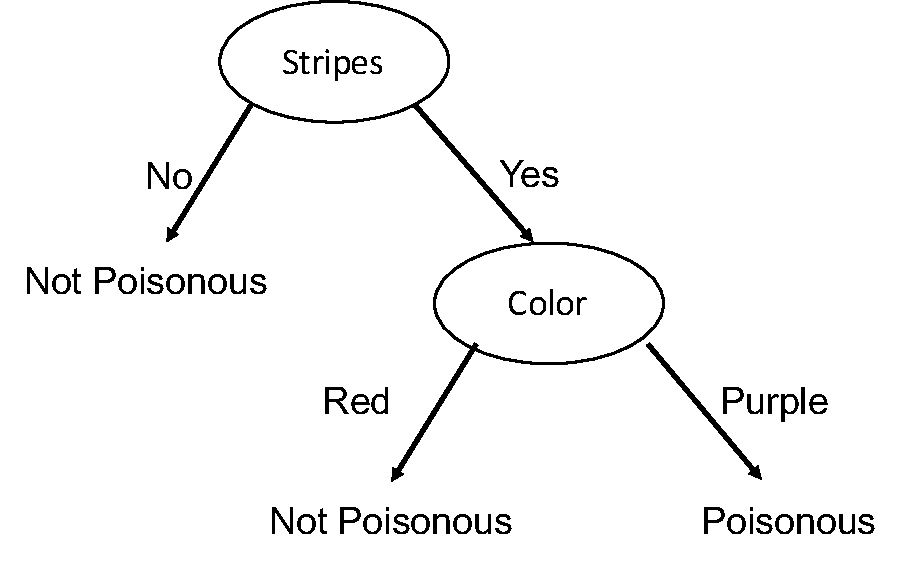
\includegraphics[width=0.45\textwidth]{tree.pdf}
%  \centering
%\end{figure}
%

\end{enumerate}


\end{document}
